\chapter{Wnioski}

\indent\indent Z wykresu (\ref{fig:graph_NACA_0012}) wynika, że odległość od brzegu wyznaczona metodą Poissona nie odbiega znacznie od dokładnej wartości obliczonej metodą siłową. Błąd w rejonie ostrza profilu można powiązać ze słabą jakością utworzonej tam siatki. Jest to również widoczne w rejonie noska i ostrza dla profilu o wygiętej szkieletowej \textsf{NACA 8207} (wykres \ref{fig:graph_NACA_8207}).

\begin{table}[h]\footnotesize
  \caption{Porównanie czasów wykonania metody siłowej i Poissona dla profili użytych w projekcie}
  \label{tab:comparision}
  \centering
\begin{tabular}{|c|c|c|}
\hline 
\rowcolor{light-gray} Metoda & NACA 0012 & NACA 8207 \\ 
\hline 
Siłowa  & 0.8 s & 2.1 s \\ 
\hline 
Równanie Poissona & 24 s & 30 s \\ 
\hline 
Ilość iteracji & 208 & 168 \\
\hline
Dokładność rozwiązania iteracyjnego & 0,09 & 0,07 \\
\hline\hline
\rowcolor{light-gray} Równanie Poissona & Czas & Iteracje\\
		\hline
		1) zerowy wektor początkowy & 24 s & 208 \\ 
		\hline
		2) dobrany wektor początkowy & 2.7 s & 14 \\
		\hline
\end{tabular} 
\end{table}

\indent Głównym mankamentem rozwiązania otrzymanego metodą Poissona jest czas wykonywania obliczeń, o rząd wielkości większy od rozwiązania siłowego (tab. \ref{tab:comparision}). Remedium jest spostrzeżenie, iż interesującym nas obszarem dokładnego rozwiązania jest bliskie sąsiedztwo brzegu profilu. Jeżeli udałoby się rozwiązać układ macierzowy w mniejszej liczbie iteracji, nie pogarszając przy tym wyników blisko brzegu, to zaoszczędzilibyśmy znaczną ilość czasu obliczeniowego. Taka możliwość istnieje, jeżeli zdefiniujemy wektor początkowy dla algorytmu iteracyjnego, o wartościach "z grubsza" odpowiadających rozkładowi rozwiązania w przestrzeni fizycznej\footnote{W programie zostało to zaimplementowane jako zainicjalizowanie zmiennej $\phi_i$ wartością \mbox{$i\cdot mod(n)\cdot \Delta$}}. Czas obliczeń  zbliża się wtedy do czasu wykonania metody siłowej (tab. \ref{tab:comparision}), a rozwiązanie w interesującym nas obszarze pozostaje poprawne (wykres \ref{fig:graph_NACA_0012_guess}).

\begin{figure}[h] 
	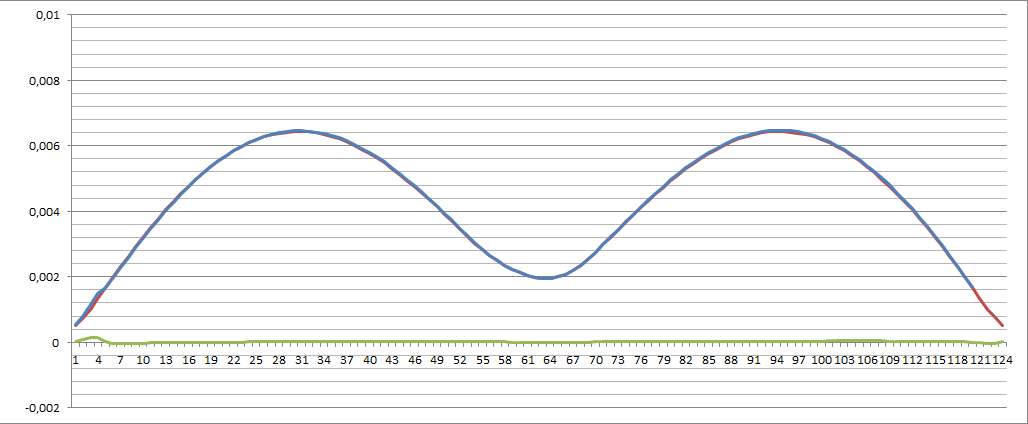
\includegraphics[trim = 30mm 0mm 0mm 0mm, width=1.1\linewidth]{Rysunki/NACA_0012_wykres_odleglosci_guess.png}
	\caption{Wykres odległości dla pierwszego rzędu siatki dla metody Poissona z \colorbox{red!30}{dobranym} wektorem początkowym i \colorbox{blue!30}{zerowym} (NACA 0012). Kolorem zielonym oznaczono \colorbox{green!30}{błąd bezwzględny}.}
	\label{fig:graph_NACA_0012_guess}
\end{figure}

\begin{figure}[H]	
    \centering
    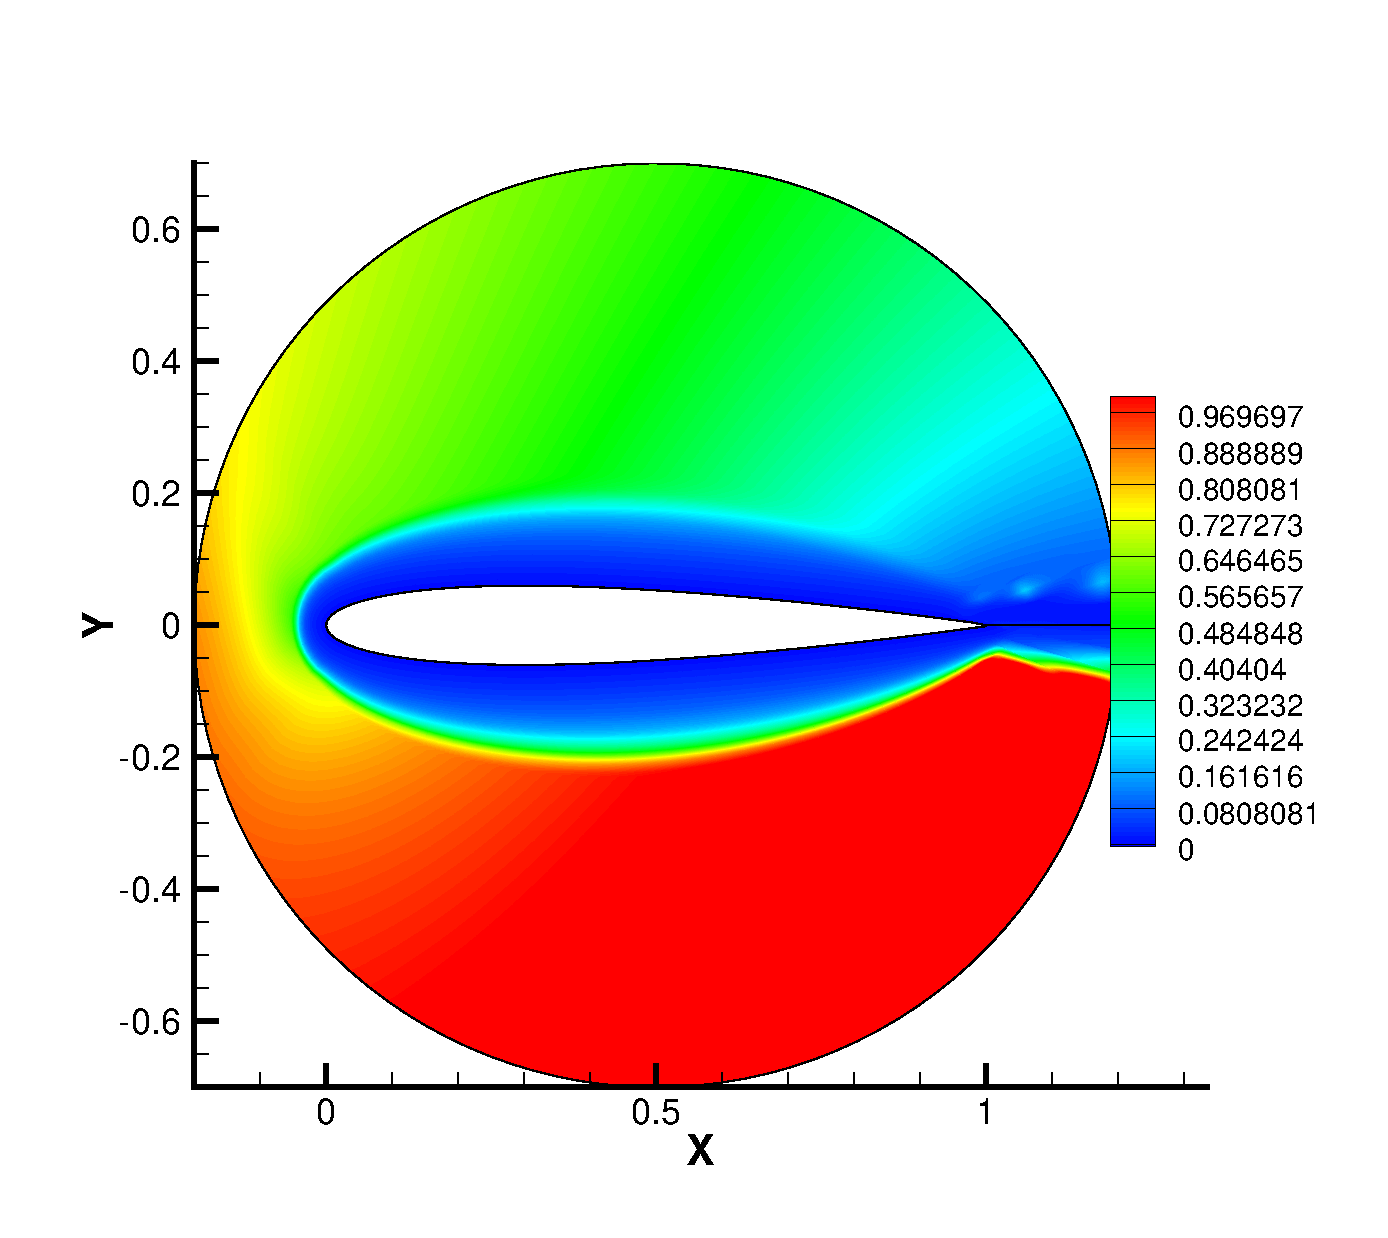
\includegraphics[trim = 22mm 10mm 10mm 20mm, width=0.9\linewidth]{Rysunki/NACA_0012_profil_poisson_guess.eps}    
	\caption{Rozwiązanie metodą Poissona otrzymane przy wykorzystaniu wektora początkowego}
\end{figure}

\section{Propozycje dalszego rozwoju}

\begin{enumerate}
	\item Jak wspomniano wcześniej, wybór iteracyjnej metody rozwiązania \mbox{\textsf{BiCSTAB}} związany był z dostępnością jej implementacji w bibliotece \textsf{Eigen}. Istnieją jednak dedykowane metody rozwiązania równania Poissona, które mogą przyspieszyć czas wykonywania programu. Jedną z nich jest \textsf{Fast Poisson Solver}, szerzej opisany w książce \textsf{Saada}\footcite{Saad, s. 58}.
	\item W oparciu o istniejącą architekturę programu należałoby dodać moduł rozwiązujący zagadnienie wykorzystując równanie Eikonału. Jest to równanie różniczkowe cząstkowe typu hiperbolicznego, dodatkowo nieliniowe. Implementacja będzie wymagać odmiennego modelu matematycznego oraz sposobu rozwiązania.
	\item Zamiast generować siatkę w programie, można ją otrzymać korzystając z pomocy zewnętrznego oprogramowania do preprocesingu (np. \mbox{\textsf{Gambit}})
\end{enumerate}